\section{Problem Setup}
\subsection{Motivating Example}
To motivate our solution, we present a running example scenario that is inspired by our experimental dataset.
A medical analyst is interested in understanding the correlation between neurological data (EEG data), patient predispositions, and the onset of seizures.

\begin{example}
An analyst is given a 15-dimensional feature vector $x \in \mathbb{R}^{15}$ of electrical signals and three binary features indicating risk factors including family history, age, and gender.
The observation is a label $y\in \{0,1\}$ of whether the patient is having a seizure.
The analyst trains a linear regression on this data.

Medical records are often dirty due various problems in digitization and data integration \cite{fortunearticle}.
After model training, the analyst is informed of inconsistencies in the three binary features representing patient data.
However, the procedure to determine which patients' data are corrupted requires querying source medical records.
\end{example}

\noindent\textbf{Cleaning or No Cleaning: } The first choice the analyst needs to make is how she should address the corruption. With existing tools, the analyst has a few options: (1) she can ignore the errors and assume that the inconsistencies do not affect the results, (2) she can discard the data and assume that the errors are not correlated with the other covariates, or (3) she can clean the entire dataset and retrain her model.
These solutions pose a dichotomy where either the analyst has to face expensive data cleaning, complete retraining, or cope with potentially unreliable analysis.

\vspace{0.5em}

\begin{figure}[ht!]
\centering
 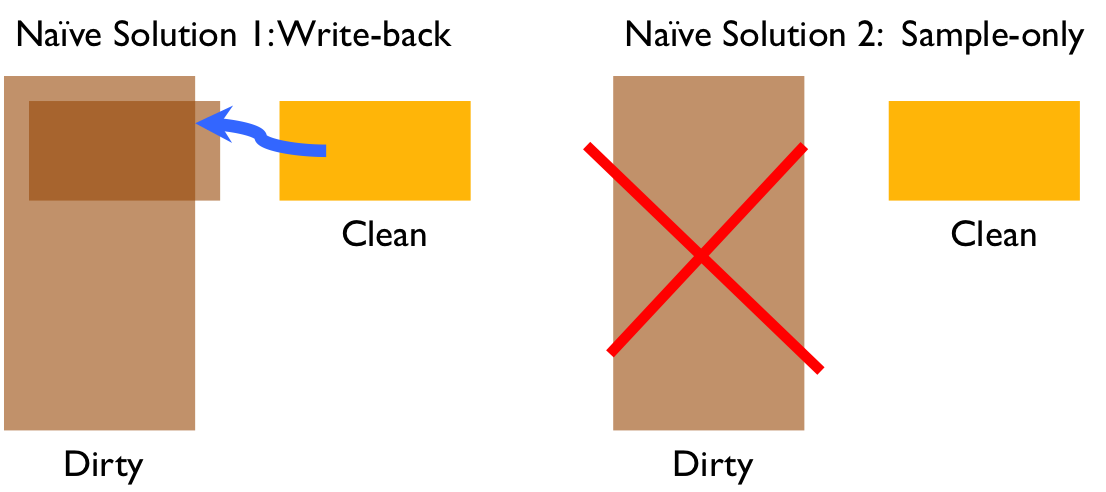
\includegraphics[width=\columnwidth]{figs/update-arch.png}
 \caption{The two naive solutions to the problem: writing-back the cleaned data, and training only on the sample. Writing back to the cleaned data potentially creates unreliable mixtures of data, and training only on the sample creates an issue of dimensionality and sample size. \label{update-arch1}}
\end{figure}

\noindent\textbf{Cleaning With a Budget: } The best choice for the analyst is determined by the systematic nature of the errors. The best scenario is if the errors are not systematic (i.e., corruption affects all patients randomly), then she can just discard the corrupted data without any expensive repair options. 
However, she cannot know this with cleaning the data.
Let us suppose our analyst wants to quickly evaluate whether the errors are systematic, and we have a budget of cleaning $k \ll N$ records of data.
The first solution to this problem (Figure \ref{update-arch1}a) is to clean a sample of data, write this sample back, and then retrain the model on the partially cleaned data.
While this solution is guaranteed to be asympotically consistent (i.e., if we clean all the data we are guaranteed the correct solution), the performance of intermediate models can be very unreliable.
In statistics, there is a well-known phenomenon called Simpsons paradox, where mixtures of different populations of data can actually result in reversed trends.

So if mixing dirty and clean data is not the correct solution, the next approach would be to neglect the dirty data altogether (Figure \ref{update-arch1}b).
SampleClean\cite{wang1999sample} approximates the results to aggregate queries by applying them to a clean sample of data.
For Machine Learning, we could train a model only on the clean sample of data.
This solution is also guaranteed to be consistent, and intermediate results are meaningful since they only reflect the clean data.
However, the problem here is that high-dimensional models are very sensitive to the sample size.
If our cleaning budget is small, sampling errors will dominate any reductions in data error.
The consequence is that we will not be able to differentiate between data error and sampling error.

\begin{example}
\textbf{Write-back.} Our analyst corrects 10 incorrect records and retrains her model on the new dataset.

\noindent \textbf{SampleClean.} Our analyst takes a sample of 10 records at random, corrects the records if incorrect, and trains her model only on the sample.

\end{example}

\vspace{0.5em}

\begin{figure}[t]
\centering
 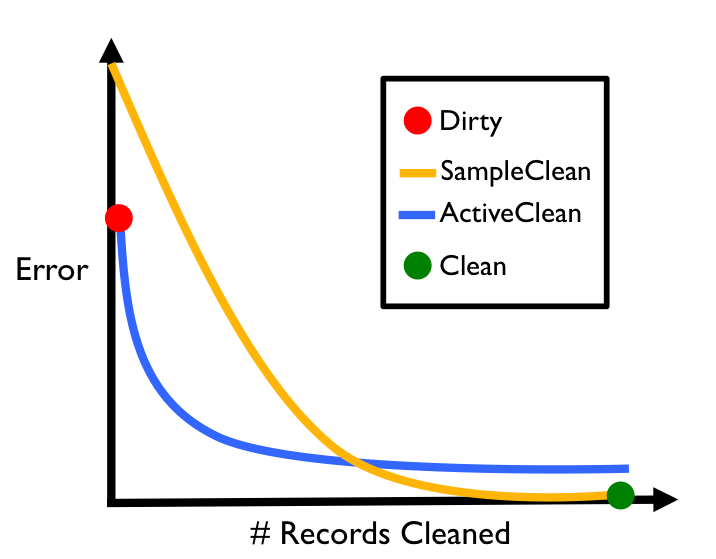
\includegraphics[width=0.6\columnwidth]{figs/arch2.png}
 \caption{\sysfull starts with a dirty model and tries to iterative correct the error in batches. In many datasets, this leads to an improved convergence rate over naive uniform sampling. \label{sys-arch2}}
\end{figure}

\noindent\textbf{The Need for \sys: } In designing \sys, we try to get the best of both worlds. We want the correctness on intermediate results given SampleClean, but we also want to avoid the strong dependence on sample size. In Figure \ref{sys-arch2}, we illustrate the tradeoff space of sampling and data cleaning.
At two extremes we have no cleaning (just using the dirty data) and full cleaning.
We argue that the naive approach of uniform sampling is not suited for Machine Learning (SampleClean) because it struggles at small sample sizes.
We design \sys to make greater progress at these small sample sizes using the dirty model as an initialization.
Doing so is not trivial since it requires analysis of both the Machine Learning model and the data cleaning operations.
Data may look unimportant to a dirty model but when cleaned are very important.
Also, data cleaning and model training can happen at very different time scales, we have to carefully budget our effort to ensure that any optimizations actually address rate-determining steps in the workflow.
Finally, in this line of work, the tradeoff space is enormous, and we have to carefully pick a design point and tailor our optimizations to this preferred regime.

\subsection{Preliminaries}
There have been a few proposals of tighter integration of data cleaning and analytics.
In SampleClean \cite{wang1999sample}, the authors formalize the analytics in terms of a SQL aggregate query.
Bergman et al. explore the problem of query-oriented data cleaning \cite{bergman2015query}, where a conjunctive query (CQ) guides which records are to be cleaned.
SQL and CQ formalize a declarative problem specification in database research.

In this paper, when we refer to Machine Learning, we are refering to a class of problems called Empirical Risk Minimization (ERM).
In a loose analogy to the declative queries in databases, loss functions in serve the same purpose in ERM.
In ERM, the goal is to learn a set of model \emph{parameters} $\theta$ from training examples.
We start with a set of training examples $\{(x_{i},y_{i})\}_{i=1}^{N}$
on which we minimize an loss function $\phi$ (a penalty for getting the prediction wrong) at each point parametrized that is parametrized by $\theta$.
\[
 \theta^{*}=\arg\min_{\theta}\sum_{i=1}^{N}\phi(x_{i}^T\theta,y_{i})
\]
For example, in a linear regression $\phi$ is:
\[
\phi(x_{i}^T\theta,y_{i}) = \|\theta^Tx_{i} - y_i \|_2^2
\]
Typically, a \emph{regularization} term $r(\theta)$ is added to this problem.
The regularization term $r(\theta)$ is traditionally what is used to increase the robustness of the model.
$r(\theta)$ penalizes high or low values of feature weights in $\theta$ to avoid overfitting to noise in the
training examples.
\[
 \theta^{*}=\arg\min_{\theta}\sum_{i=1}^{N}\phi(x_{i}^T\theta,y_{i}) + r(\theta)
\]
For example, a popular variant of linear regression is called LASSO which is:
\[
 \theta^{*}=\arg\min_{\theta}\sum_{i=1}^{N}\|\theta^Tx_{i} - y_i \|_2^2 + \lambda \cdot \|\theta\|_1
\]
By applying the L1 regularization term, if one of the features is particularly noisy, and does not add predictive value, it will get excluded.
The loss function specifies a problem independent of the optimization used to calculate the optimal parameter $\theta^{*}$.

A very important class of problems is when $\phi$ and $r$ are convex in $\theta$.
Convex problems are amenable to a variety of different optimization methodologies
and have strong theoretical guarantees on convergence rates.
This class of problems includes all generalized linear models (including linear and logistic regression), and all variants of support vector machines.
In this work, we focus on this class of problems as it is very broad yet we can still analyze the results.

\subsubsection{Systematic Biases}
We explore methodologies for training models when data is systematically incorrect leading to a biased model.
In our running example, systematic errors could include:
\begin{example}\label{exm-1}
Older patients whose records were manually digitized are more likely to have missing values.
\end{example}
\begin{example}\label{exm-2}
Occurances of certain types of seizures are mislabled with more false negatives than false positives.
\end{example}
If we ignore these errors, our model may have a few different problems. 
First, consider Example \ref{exm-1}, if older patients are more likely to have record errors the model's performance of predicting the occurrance of seizures will be unreliable for that subpopulation. 
A robust model may ``overfit" to the uncorrupted data completely ignoring this corrupted population.
Next, consider Example \ref{exm-2}, mislabled data is actually a very subtle error.
The labels are a proxy for predicting a real-world phenomenon.
If we train a model with respect to the incorrect data, while we might have achieve a good out-of-sample accuracy on the incorrect data, but the classifications are incorrect in a real world sense.

The underlying problem here is that the model is trained on an incorrect data distribution.
There is a latent data distribution that represents the real world.
When these two distributions are not aligned (i.e., the training data is not an i.i.d sample from the real world), then there is no guarantee that the model will reliably generalize.
Consider example \ref{exm-1}, suppose those patients have missing values in a certain attribute.
If those patients are more likely to get seizures, the model will learn a correlation between the missing data and increased prevalance of seizures.
While this missing data has some predictive value, these incorrect inferences can lead to analysis pipelines that are brittle.
Imagine if a batch new patients also lacked the same attribute, they could be incorrectly classified due to this spurious correlation.

Essentially, this problem is of training on one distribution and testing on another.
To characterize this problem there are two metrics that we look at:

\vspace{0.5em}

\noindent\textbf{Model Error. } Let $\theta$ be the model trained on the dirty data, and let $\theta^*$ be the model trained on the same data if it was cleaned. Then the model error is defined as $\|\theta - \theta^*\|$.

\vspace{0.5em}

\noindent\textbf{Testing Error. } Let $\theta$ be the model trained on the dirty data, and let $\theta^*$ be the model trained on the same data if it was cleaned. Let $T(\theta)$ be the out-of-sample testing error when the dirty model is applied to the clean data, and $T(\theta^*)$ be the test error when the clean model is applied to the clean data. The testing error is defined as $T(\theta^*) - T(\theta)$

\begin{problem}[ActiveClean Problem]\label{activeclean}\sloppy
Let $R$ be a dirty relation and each row $r \in R$ is 
turned into a feature vector and label tuple $F(r) \mapsto (x,y)$.
We are given a convex regularized loss model parametrized
by $\theta$ trained on the set of features and labels $\{(x,y)\}$.
The user specifies two data cleaning components: (1) error detection
which selects a set of candidate dirty data $R_{dirty}$, and (2) error 
repair which cleans a record $C(r) \mapsto r_{clean}$.
With a budget of applying cleaning i.e., $C(\cdot)$, only k times, we return an estimate $\hat{\theta}$ of the clean model.
\end{problem}

\noindent Here is an example use case of \sys:
\begin{example}
Let us suppose that the EEG dataset is corrupted with the systematic errors described in Example \ref{exm-1}.
The analyst first trains her linear model on the dirty data ignoring the effects of the errors returning a model $\theta^{(d)}$.
Then, she provides ``error detection" logic, selecting a set of possibly corrupted records $R_{dirty}$ by listing all records with missing values.
She sets a desired cleaning batch size of $b=10$ and number of iterations $t=4$.
She initializes \sys with $\theta^{(d)}$ and inspects samples of 10 records from $R_{dirty}$.
She manually corrects those records by the medical record source data.
After each batch, the model is updated with the most recent result $\theta^{(t)}$.
After $t=4$ of cleaning, the analyst can evaluate the difference $\theta^{(d)}$ and the current best model $\theta^{(4)}$ to see if the data error causes a systematic bias.
\end{example}

\iffalse

\subsection{Two perspectives on error}
When faced with such errors there are two contrasting perspectives from the Machine Learning and the Database communities.

\vspace{0.5em}

\noindent\textbf{Existing Database Literature. } 
Traditionally, cleaning is agnostic to the queries and analysis that happens downstream. 
This perspective breaks down when cleaning is so expensive that we can only clean a small number of records.
Ideally, we should clean the records that are most valuable to the downstream analysis.

\vspace{0.5em}

\noindent\textbf{Existing  Machine Learning Literature. } The Machine Learning community has focused on
designing models that are robust to outliers (i.e., values far away from the typical value)
For example, in the case of linear regression, we can change the $L_2$ norm to an $L_1$ norm to mitigate the effect of outliers:
\[
\phi(x_{i}^T\theta,y_{i}) = \|\theta^Tx_{i} - y_i \|_1
\]
The quadratic L2 loss implies that examples that deviate far from the typical example are quadratically penalized as opposed to linearly penalized with the L1 loss.
There is a natural tradeoff between robustness and efficiency.
The more robust a technique is, the less efficient it will be (i.e., estimate variance for a fixed number of training examples).
Robust techniques are best suited for random errors that look significantly different the rest of the examples.
When errors are systematic, the Machine Learning answer has been to design features in such a way that they are robust to some systematic bias.
For example, in image processing, scale-invariant feature transforms (SIFT) are widely applied that allow for image models invariant to pose or scaling issues.

\vspace{0.5em}

\noindent\textbf{The \sys Contribution. } We try to bring two perspectives together in this work to address the problem of expensive to clean systematic errors, namely the Database idea of data cleaning and the Machine Learning formalization of empirical risk minimization.
Some errors require expensive cleaning procedures, increasingly using the crowd, and we joint have a time budget on cleaning and analysis.
\sys prioritizes cleaning with respect to an estimated impact on the clean model.



\subsection{SampleClean Project}

Traditionally, data cleaning has explored expensive, up-front cleaning of entire datasets for increased query accuracy.
We proposed the SampleClean problem, in which an analyst cleans a small sample of data, and then estimates the result to an aggregate query e.g., \sumfunc, \countfunc, or \avgfunc.
The main insight from the SampleClean project is that highly accurate answers for aggregate queries does not require cleaning the full dataset.
Generalizing this insight, there is a deep relationship between the application (i.e., the query) and how an analyst should budget their effort in data cleaning.
In fact, \avgfunc and \sumfunc queries are a special case of the convex loss minimization discussed in the previous section:
\[
\phi = (x_{i} - \theta)^2
\]

We then extended the SampleClean work to study cleaning Materialized Views \cite{technicalReport}.
Suppose base data is updated with insertions, deletions, or updates, we explored how we could efficiently propagate
changes to a sample of the view instead of the full view.
Subsequent queries on the view could be answered approximate.

The SampleClean problem inspired an eponymous system that implements sampling, data cleaning, and approximate query processing on the Apache Spark stack \cite{sampleclean}.
Also included in the Apache Spark stack are Machine Learning libraries including MLlib \cite{mllib} and GraphX \cite{graphx}.
The in-memory architecture of the Apache Spark stack allows for increasingly interactive analysis \cite{AgarwalMPMMS13, armbrust2015spark}.
Analysts can prototype data processing workflows on samples to evaluate performance before running expensive batch processing jobs on entire datasets.
With data cleaning and machine learning libraries in the same software ecosystem, we see a new opportunity for joint optimization for interactive model building.



\subsection{Stochastic Gradient Descent}
Sampling is a natural part of any Machine Learning workflow, as stochastic optimization is widely used to fit model parameters.
The problems described in the previous subsections are often trained using a technique called Stochastic Gradient Descent (SGD) or one of its variants.
The basic idea of SGD is to draw a data point at random, calculate the gradient at that point, and then update a current best estimate with that gradient.
\[
\theta^{(t+1)}\leftarrow\theta^{(t)}-\gamma\nabla\phi(x_{i}^T\theta,y_{i})
\]
 SGD can also be applied in a ``mini-batch" mode, where we draw a subset of data $S^{(t)}$ at random and update with the average gradient.
 \[
 \theta^{(t+1)}\leftarrow\theta^{(t)}-\frac{\gamma}{\|S^{(t)}\|}\sum_{i\in S^{(t)}}\nabla\phi(x_{i}^T\theta,y_{i})
 \]

We can use this workflow for designing an anytime data cleaning methodology.
As data is sampled, we can clean the samples.
The analyst then can stop at anytime and use the best model at that instant.
SGD and its variants are well-studied and there are lower-bounds on the convergence rates using these techniques. 
Recently, a number of works have explored non-uniform sampling distributions for stochastic optimization \cite{zhao2014stochastic, qu2014randomized}.
The main insight is that non-uniform distributions may on average estimate the gradient accurately.
In this work, we explore how to design such a non-uniform distribution for iterative data cleaning.

\fi


 